% !TEX TS-program = xelatex
\documentclass[12pt,a4paper]{article}
\usepackage{fontspec}\usepackage{polyglossia}
\setmainlanguage{english}\setotherlanguage{russian}
\setmainfont{DejaVu Serif}\setsansfont{DejaVu Sans}\setmonofont{DejaVu Sans Mono}
\usepackage[a4paper,margin=2.05cm]{geometry}
\usepackage{amsmath,amssymb,mathtools,graphicx,booktabs,longtable,array,hyperref,float,enumitem,microtype}
\hypersetup{colorlinks=true,linkcolor=blue,urlcolor=blue}
\setlength{\parskip}{0.52em}\setlength{\parindent}{0pt}\renewcommand{\arraystretch}{1.12}\sloppy

\title{\textbf{Computational Validation of Adaptive Interface Control in TMI Quantum Systems}\\\large Extended v5 report on Tests 1--28}
\author{Salkutsan Aleksey}\date{May 7, 2026}\begin{document}\maketitle
\begin{abstract}
This report extends the TMI computational validation line to Tests 1--28. Version v5 adds Test 28: out-of-distribution Qiskit-Aer generalization on unseen circuit families that were not used in calibration. The main new result is:
\[Calibrate(I_{sim})\land Correct(I_{circuit})\Rightarrow Generalize(C_{new}).\]
This is simulator validation, not laboratory proof of a physical theory.
\end{abstract}\tableofcontents\newpage
\section{Report status}
\[\boxed{\text{TMI Quantum Computational Validation v0.5}}\]

\section{Summary of Tests 1--28}
\begin{longtable}{p{0.9cm}p{4.0cm}p{5.0cm}p{5.4cm}}
\toprule
Test & Name & Criterion / meaning & Result \\
\midrule
\endfirsthead
\toprule
Test & Name & Criterion / meaning & Result \\
\midrule
\endhead
1 & Ramsey toy model & T2\_TMI > T2\_standard & Delta T2 = 58.1 us \\
2 & Noisy Ramsey learning & T2\_TMI > T2\_standard & Delta T2 = 39.3 us \\
3 & Small quantum circuit & P\_TMI > P\_standard & Delta P = 0.115 \\
4 & Stabilized interface & Stable adaptive control & Delta P = 0.026 \\
5 & Surrogate Monte Carlo & E[P\_TMI] > E[P\_standard] & Delta = 0.0510, Pr = 0.864 \\
6 & Ablation study & Structured adaptive control & full TMI Delta = 0.0680 \\
7 & Density-matrix Monte Carlo & Full matrix validation & Delta = 0.0930, Pr = 0.933 \\
8 & Cross-model validation & Multiple circuit families & Delta = 0.0660, Pr = 0.846 \\
9 & Failure-boundary map & Weak/failure regions & failure = 0, weak = 6 \\
10 & Adversarial failure & Forced failure modes & failure cells = 58 \\
11 & Safety recovery & Mitigation after failure & recovered = 31/58 \\
12 & Reproducibility harness & One-command validation & passed = 11/11 \\
13 & Independent simulator & Independent simulator validation & Delta = 0.1121, Pr = 1.000 \\
14 & Noise-model stress & Noise class robustness & passed = 3/4, Delta = 0.0068 \\
15 & Amplitude damping recovery & Relaxation-aware layer & Delta\_relax = 0.1532 \\
16 & Noise classifier & Classify then control & accuracy = 0.952, Delta = 0.0554 \\
17 & Online noise drift & Dynamic reclassification & Delta = 0.0255, acc = 0.816 \\
18 & Delayed feedback & Latency hurts online control & online = 0.883, delayed d2 = 0.861 \\
19 & Latency policy optimization & Predictive latency layer & opt = 0.875 > d2 = 0.861 \\
20 & Cost-overhead tradeoff & Utility and efficiency & U\_highperf = 0.0705 \\
21 & Cost-interface boundary & B\_cost & lambda* = 0.0636 \\
22 & Multi-objective control & Boundary manifold & standard share = 0.608, cost-aware-low = 0.373 \\
23 & Standard simulator protocol & Backend-independent Qiskit-style protocol & Delta = 0.0414, Pr = 0.750 \\
24 & Raw Qiskit-Aer execution & External simulator without calibration & failed, Delta = -0.00097, cells = 0/16 \\
25 & Qiskit noise calibration & Simulator-interface calibration & 54 candidate calibrations; Loss\_sim = 0.00106 \\
26 & Calibrated Qiskit-Aer validation & Held-out calibrated validation & passed, Delta = 0.0725, cells = 12/16 \\
27 & Circuit-inverse audit & Correct inverse and rerun Qiskit-Aer & passed, Delta = 0.1144, cells = 16/16 \\
28 & OOD Qiskit-Aer generalization & Unseen circuit families & passed, Delta = 0.1252 to 0.1414, cells = 24/24 \\
\bottomrule
\end{longtable}

\section{External Qiskit-Aer branch: failure, calibration, correction, generalization}

The external branch now has the following structure:
\[
Test\ 24:\ failed\to Test\ 25:\ calibrated\to Test\ 26:\ passed\to Test\ 27:\ corrected\to Test\ 28:\ OOD\ passed.
\]

\subsection{Test 24: raw Qiskit-Aer failure}
\[
P_{base}=0.7535,\quad P_{standard}=0.7532,\quad P_{TMI}=0.7523.
\]
\[
\Delta(P_{TMI}-P_{standard})=-0.00097,\quad cells=0/16.
\]

\subsection{Test 25: simulator-interface calibration}
Test 25 found 54 candidate calibrations and introduced the diagnostic concept:
\[
I_{sim}:TMI\ model\to Qiskit\ NoiseModel,\qquad Loss_{sim}(I_{sim})>0.
\]
In the default-like calibrated regime:
\[
\Delta(P_{standard}-P_{base})=0.0191,\quad
\Delta(P_{TMI}-P_{standard})=0.0299.
\]

\subsection{Test 26: calibrated Qiskit-Aer validation}
\[
P_{base}=0.4793,\quad P_{standard}=0.5203,\quad P_{TMI}=0.5928.
\]
\[
\Delta(P_{TMI}-P_{standard})=0.0725,\quad cells=12/16.
\]

\subsection{Test 27: circuit-inverse audit}
Original circuits failed ideal inverse correctness; corrected circuits passed. The key fix was:
\[
\texttt{S}\to\texttt{Sdg},\qquad S^{-1}=S^\dagger.
\]
After correction:
\[
P_{base}=0.5791,\quad P_{standard}=0.6432,\quad P_{TMI}=0.7576.
\]
\[
\Delta(P_{TMI}-P_{standard})=0.1144,\quad cells=16/16.
\]

\subsection{Test 28: out-of-distribution Qiskit-Aer generalization}
Test 28 used unseen circuit families, not used in calibration or correction. The conservative uploaded profile gives:
\[
P_{base}=0.2914,\quad P_{standard}=0.3424,\quad P_{TMI}=0.4616.
\]
\[
\Delta(P_{standard}-P_{base})=0.0511,\quad
\Delta(P_{TMI}-P_{standard})=0.1191.
\]
\[
Pr(P_{TMI}>P_{standard})=1.0,\quad cells=24/24.
\]
Across reported OOD profiles, all passed:
\[
\texttt{best\_by\_channel},\quad \texttt{conservative},\quad \texttt{stress\_high\_signal}.
\]

\section{Visual summary}
\begin{figure}[H]\centering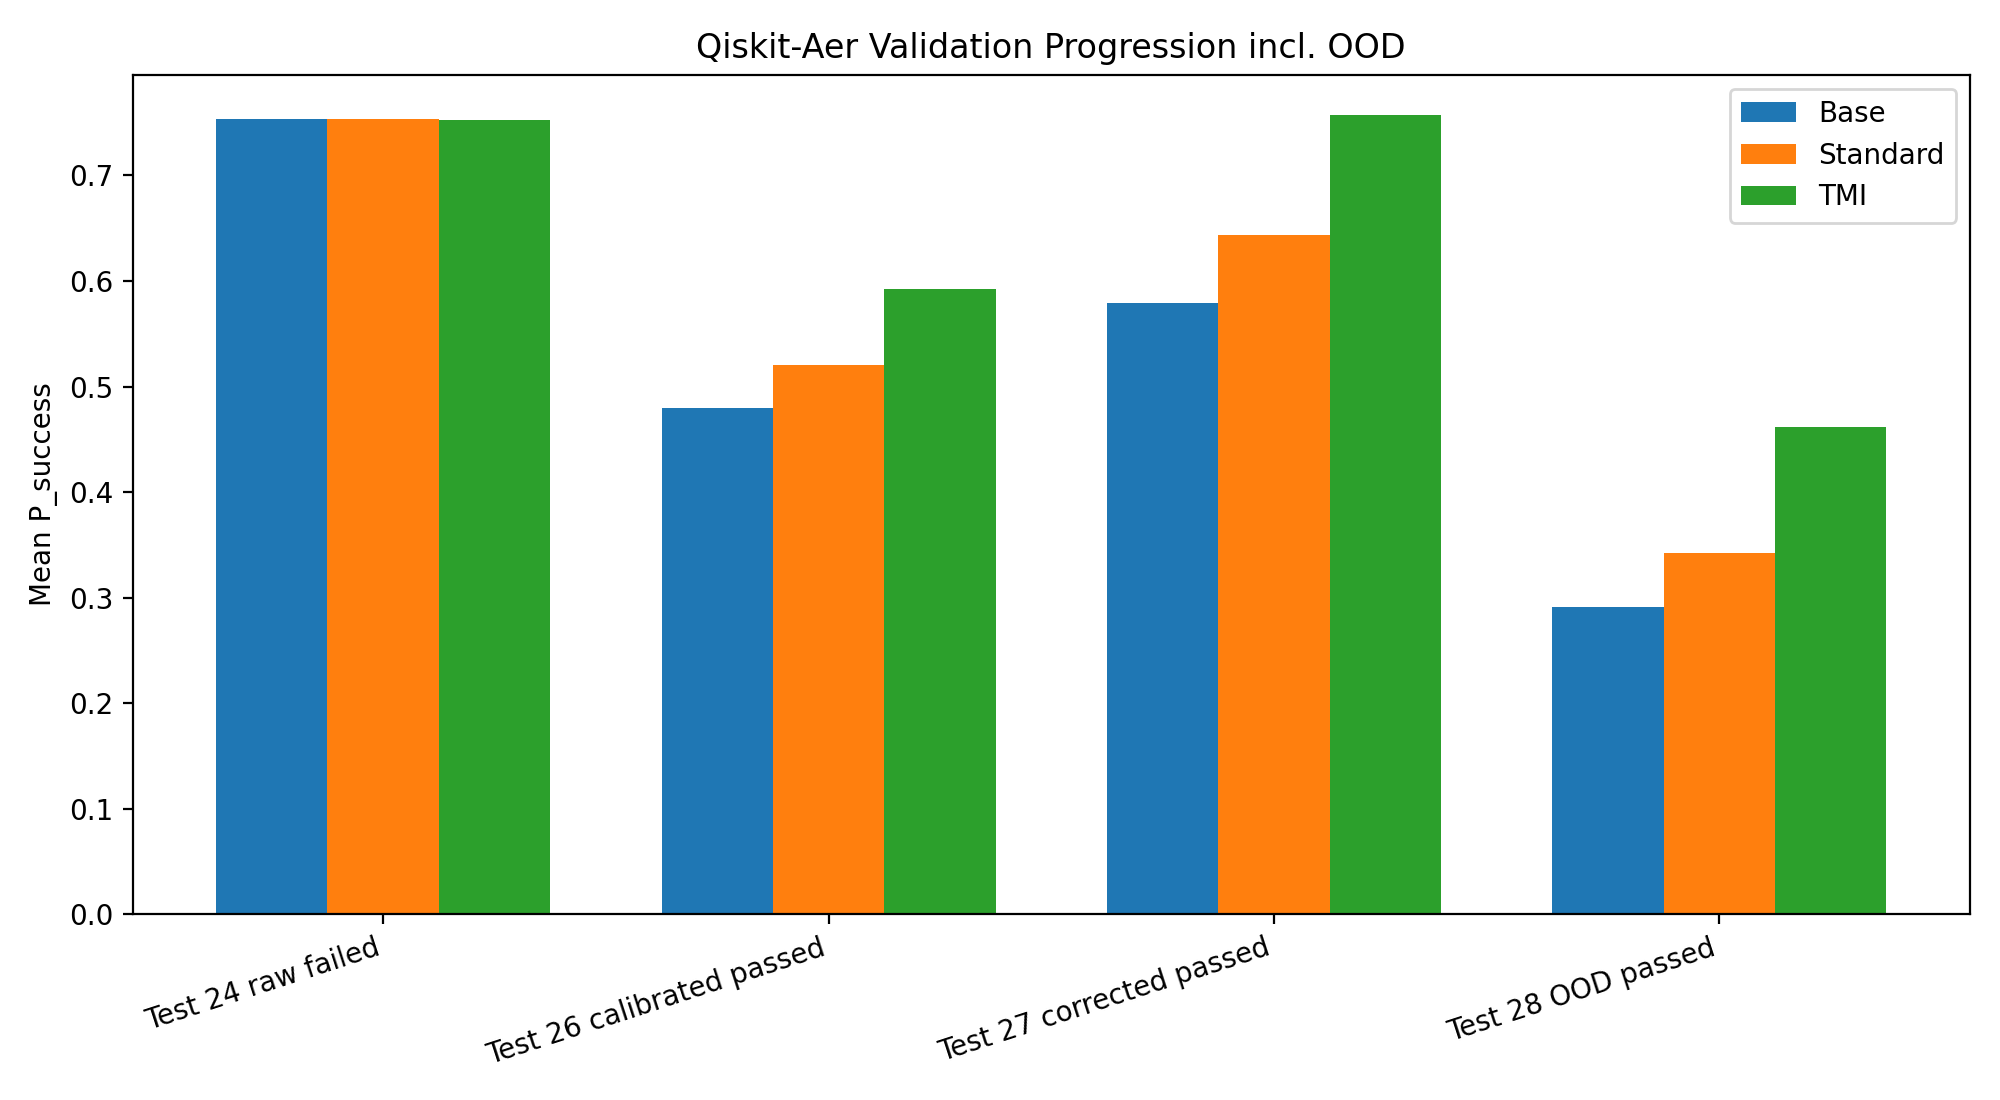
\includegraphics[width=0.88\linewidth]{figures/fig_v5_qiskit_ood_progression_mean_p.png}\caption{External Qiskit-Aer progression including OOD generalization.}\end{figure}
\begin{figure}[H]\centering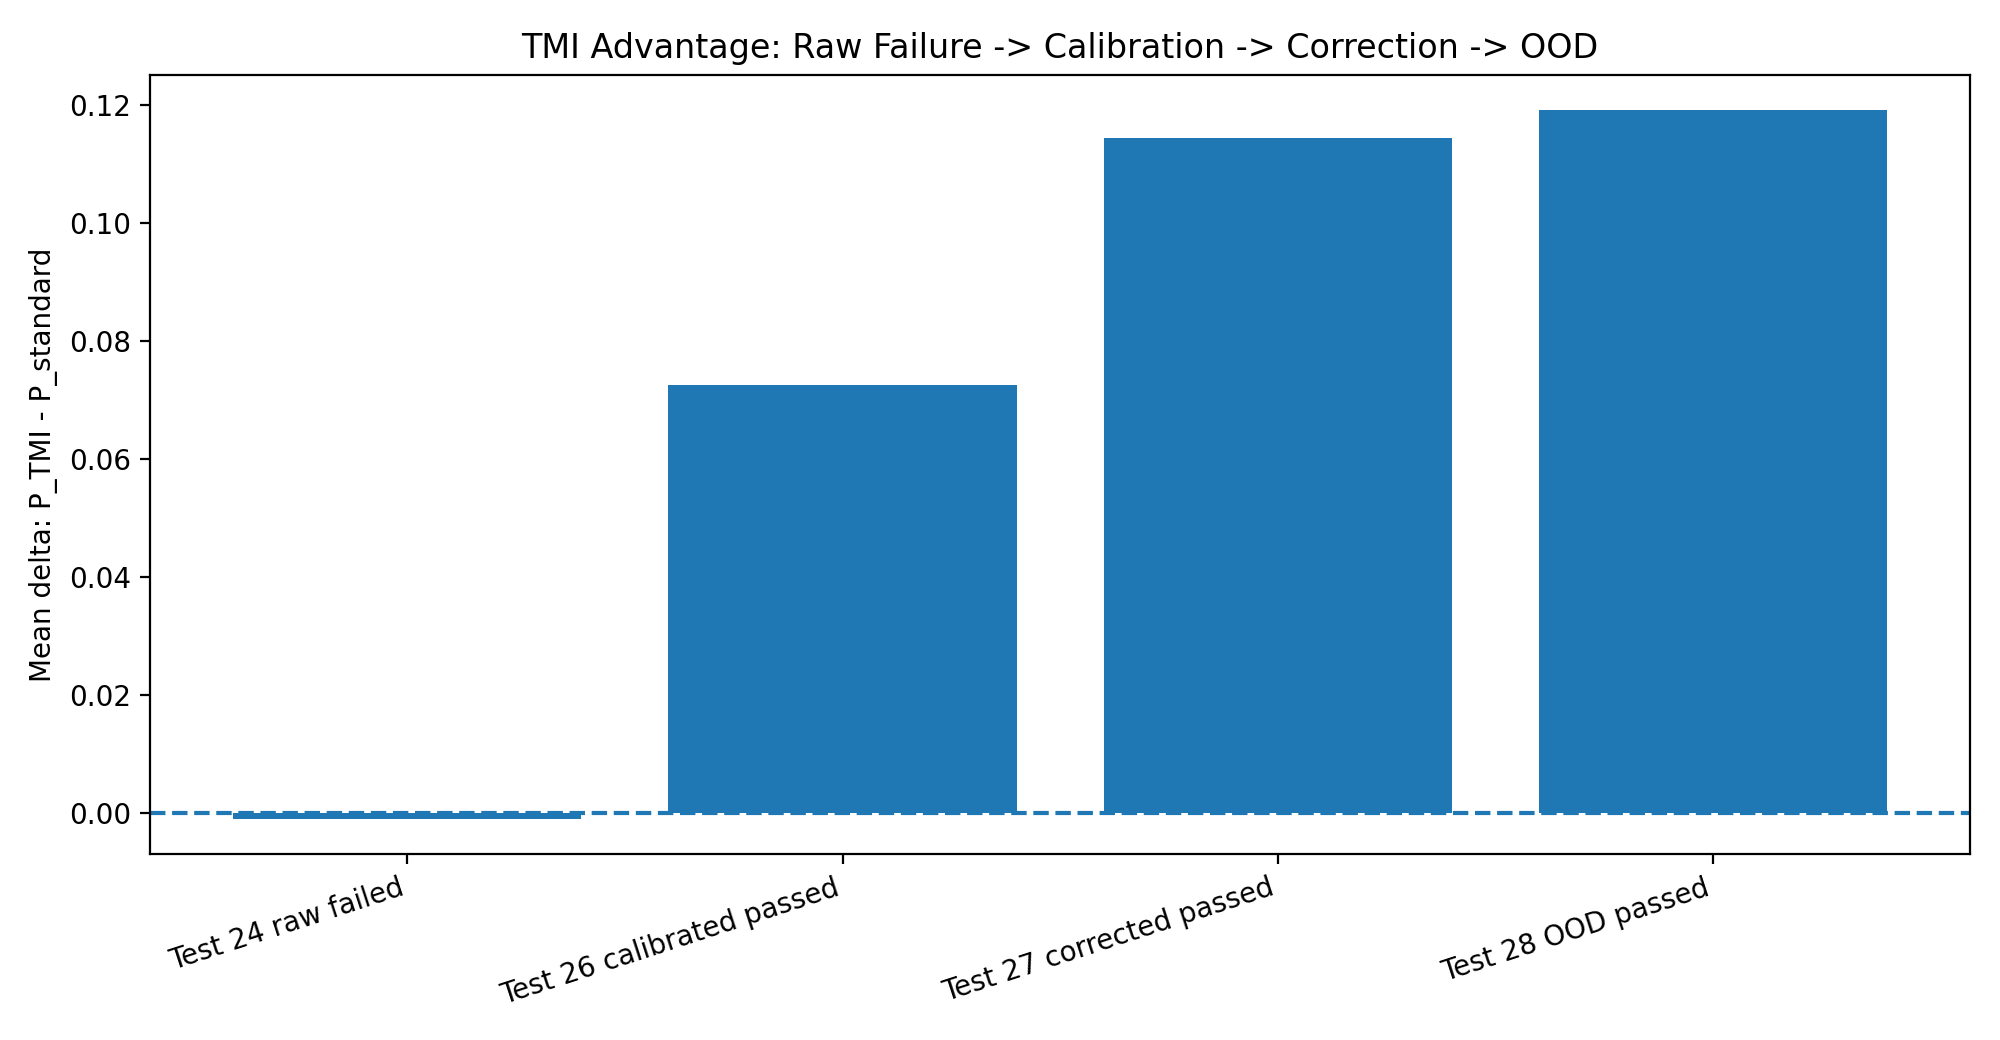
\includegraphics[width=0.88\linewidth]{figures/fig_v5_qiskit_ood_delta_progression.png}\caption{$P_{TMI}-P_{standard}$: raw failure becomes positive after calibration, correction and OOD validation.}\end{figure}
\begin{figure}[H]\centering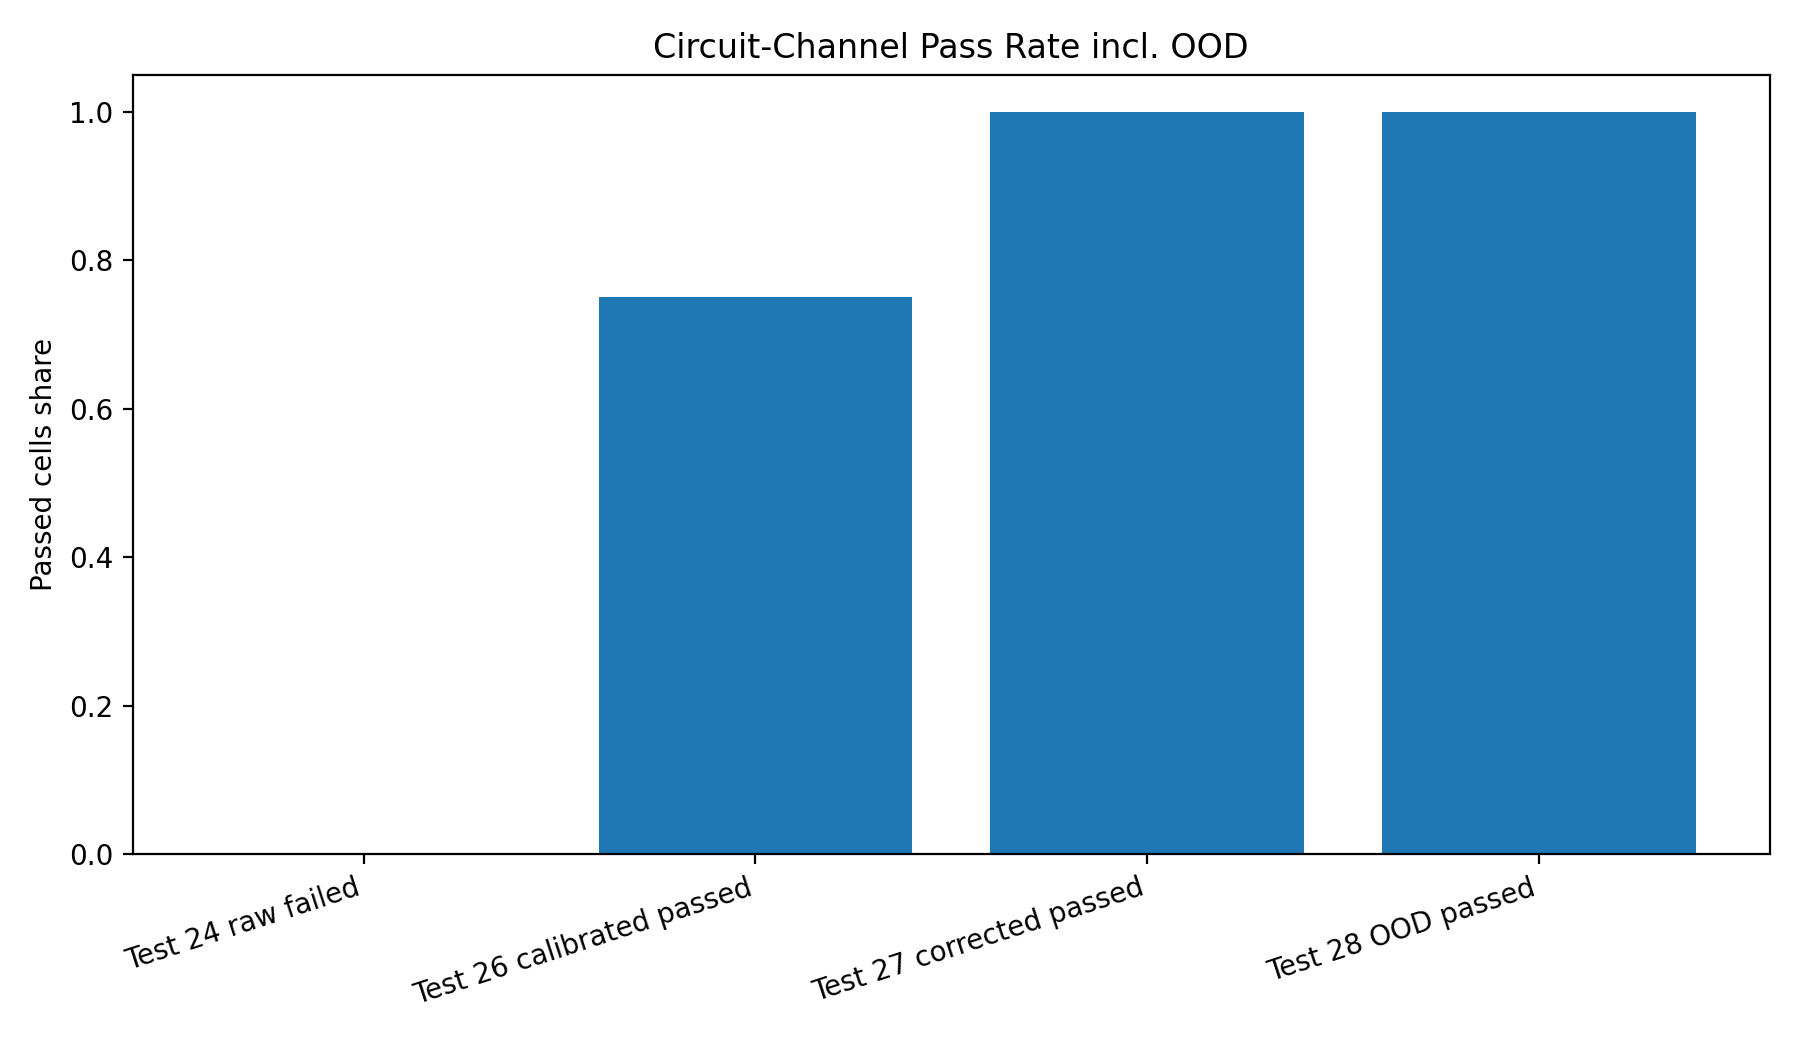
\includegraphics[width=0.82\linewidth]{figures/fig_v5_cells_pass_rate.png}\caption{Cell pass rate: 0/16, 12/16, 16/16, 24/24.}\end{figure}
\begin{figure}[H]\centering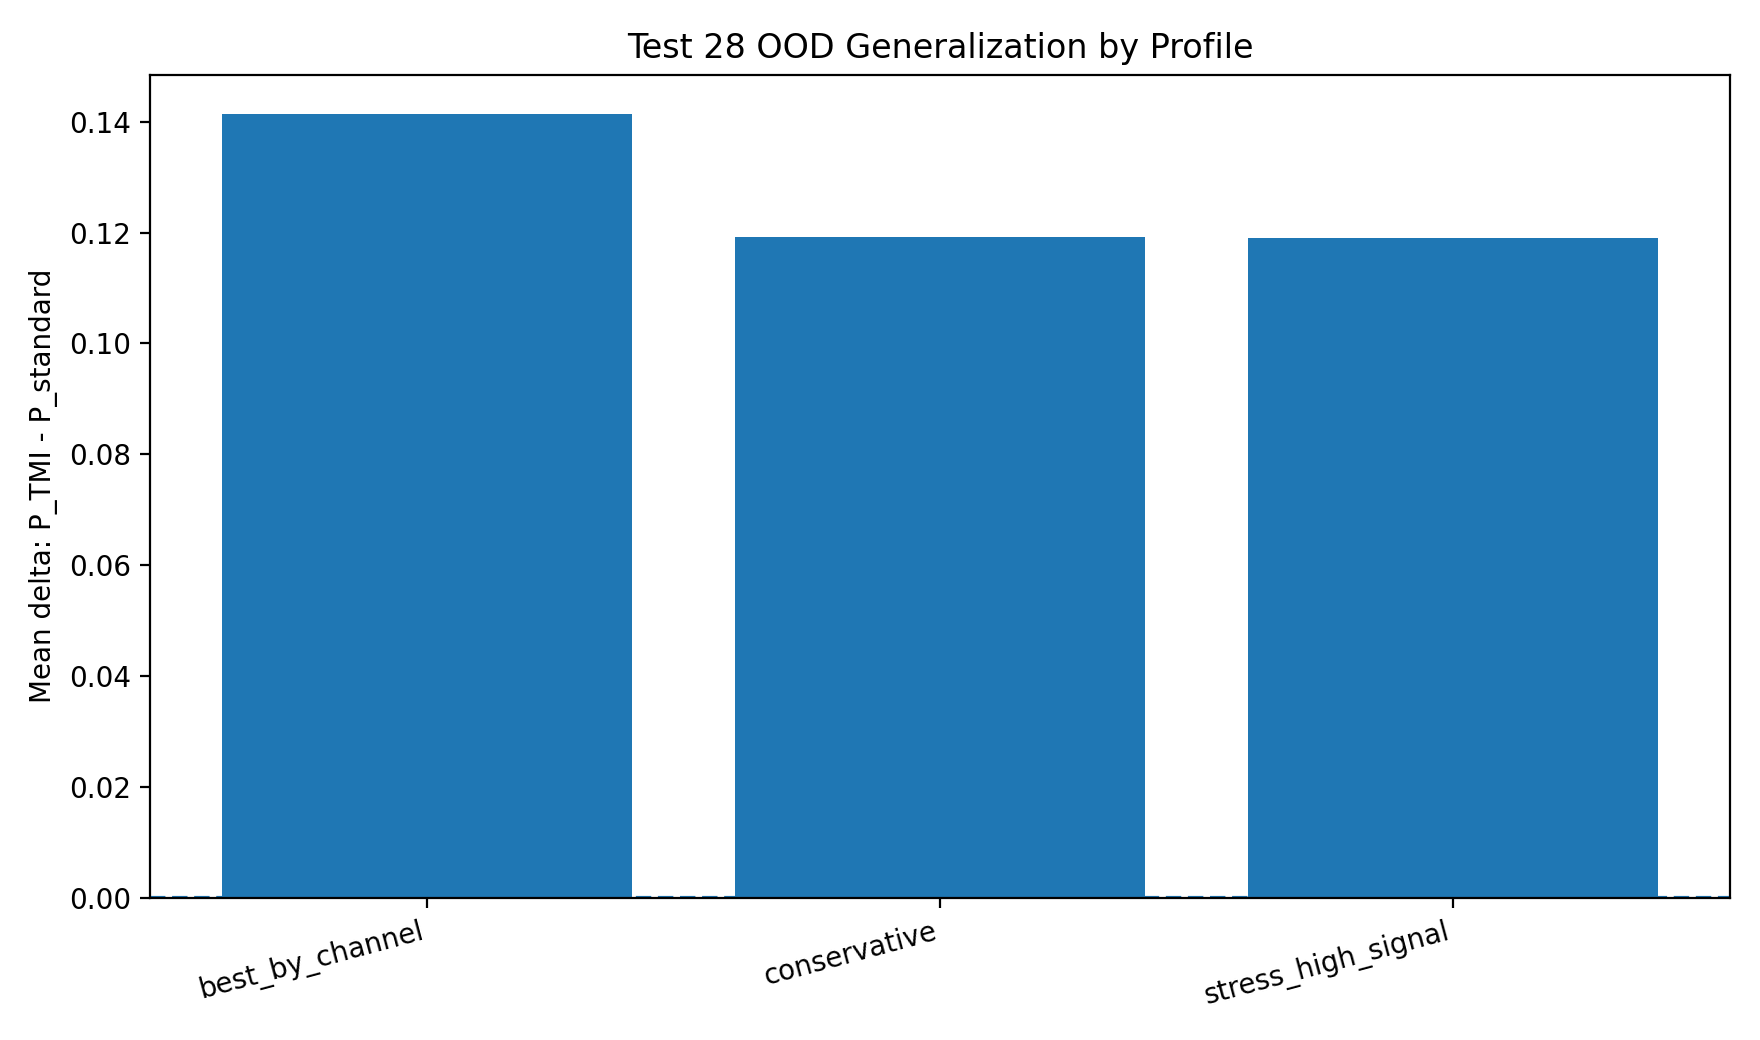
\includegraphics[width=0.76\linewidth]{figures/fig_v5_test28_profile_deltas.png}\caption{Test 28 OOD deltas by profile.}\end{figure}

\section{v5 formulas}
\[
\boxed{Calibrate(I_{sim})\land Correct(I_{circuit})\Rightarrow Generalize(C_{new})}
\]
\[
\boxed{C_{new}\notin C_{calibration}\Rightarrow P_{TMI}>P_{standard}>P_{base}}
\]

\section{Conclusion}
Version v5 adds out-of-distribution Qiskit-Aer generalization. The result is stronger than v4 because it shows that the calibrated/corrected simulator-interface mechanism is not limited to the circuit families used in calibration.

\appendix\section{Package contents}
The package contains Russian and English PDF/LaTeX sources, JSON/CSV summaries, external Qiskit-Aer branch figures, Tests 12--28 packages, and Tests 24--28 status files.
\end{document}
